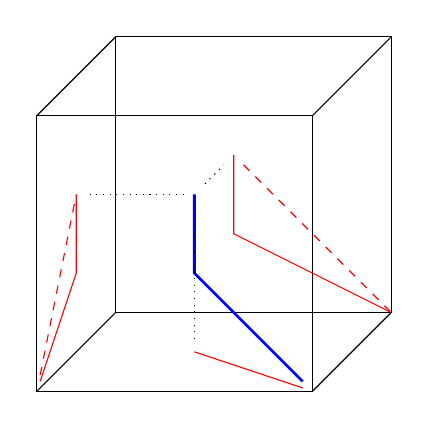
\begin{tikzpicture}
\tikzstyle{visited}=[line width=1pt,blue];

\draw  (-2.5,1.5) node (v2) {} rectangle (1,-2) node (v4) {};
\draw  (-1.5,2.5) node (v1) {} rectangle (2,-1) node (v3) {};
\draw (1,1.5) -- (2,2.5);
\draw (-1.5,-1) node (v7) {} -- (-2.5,-2) node (v9) {};
\draw (2,-1) node (v10) {} --  (1,-2) node (v5) {};
\draw  (-1.5,2.5) node (v8) {} --  (-2.5,1.5) ;


\draw[blue,line width=1pt] (-0.5,0.5) node (v12) {} -- (-0.5,-0.5) -- (0,-1) -- (v5);
\draw[red] (0,1) node (v6) {} -- (0,0) -- (2,-1);
\draw[red] (-0.5,-1.5) node (v13) {} -- (v5);
\draw[red] (-2,0.5) node (v11) {} -- (-2,-0.5) -- (v9);
\draw[red, dashed] (v6) -- (2,-1);
\draw[red, dashed] (v11) -- (v9);
\draw[dotted]  (v12) edge (v6);
\draw[dotted]  (v12) edge (v11);
\draw[dotted]  (v12) edge (v13);
\end{tikzpicture}